% !TeX spellcheck = en_GB
\ifcsname SlidesDistr\endcsname%
\documentclass[handout,aspectratio=169]{beamer}
\else%
\documentclass[aspectratio=169]{beamer}
\fi%
\usepackage{fontspec}
\usepackage[T1]{fontenc}
\usepackage{amsmath}
\usepackage{amsfonts}
\usepackage{amssymb}
\usepackage{graphicx}
\usepackage{csquotes}
\usepackage{booktabs}
\usepackage{multicol}
\usepackage{enumerate}
\usepackage{microtype}
\usepackage[labelfont=bf,font={small}]{caption}
\usepackage{hyperref}
\usepackage{booktabs}
\usepackage{subcaption}
\usepackage{fancyhdr}
\usepackage{pdfpages}
\usepackage{siunitx}
\usepackage{tikz}
\usepackage{mdframed}

\defaultfontfeatures{Mapping=tex-text}
\newfontfamily\symbolfont{Symbola}
\newfontfamily\quotefont{Gentium}

\usepackage[sorting=none]{biblatex}
\addbibresource{../bibliography.bib}

\author{Andreas Stöckel}


\renewcommand{\vec}[1]{{\mathbf{#1}}}
\newcommand{\mat}[1]{{\mathbf{#1}}}
\newcommand{\T}{\ensuremath{\mathsf{T}}}
\renewcommand{\epsilon}{\varepsilon}
\renewcommand{\phi}{\varphi}

% Tango color palette
\definecolor{butter1}{HTML}{FCE94F}
\definecolor{butter2}{HTML}{EDD400}
\definecolor{butter3}{HTML}{C4A000}
\definecolor{orange1}{HTML}{FCAF3E}
\definecolor{orange2}{HTML}{F57900}
\definecolor{orange3}{HTML}{CE5C00}
\definecolor{chocolate1}{HTML}{E9B96E}
\definecolor{chocolate2}{HTML}{C17D11}
\definecolor{chocolate3}{HTML}{8F5902}
\definecolor{chameleon1}{HTML}{8AE234}
\definecolor{chameleon2}{HTML}{73D216}
\definecolor{chameleon3}{HTML}{4E9A06}
\definecolor{skyblue1}{HTML}{729FCF}
\definecolor{skyblue2}{HTML}{3465A4}
\definecolor{skyblue3}{HTML}{204A87}
\definecolor{plum1}{HTML}{AD7FA8}
\definecolor{plum2}{HTML}{75507B}
\definecolor{plum3}{HTML}{5C3566}
\definecolor{scarletred1}{HTML}{EF2929}
\definecolor{scarletred2}{HTML}{CC0000}
\definecolor{scarletred3}{HTML}{A40000}
\definecolor{aluminium1}{HTML}{EEEEEC}
\definecolor{aluminium2}{HTML}{D3D7CF}
\definecolor{aluminium3}{HTML}{BABDB6}
\definecolor{aluminium4}{HTML}{888A85}
\definecolor{aluminium5}{HTML}{555753}
\definecolor{aluminium6}{HTML}{2E3436}

\definecolor{violet}{HTML}{AA305C}
\definecolor{uwyellow}{HTML}{FDD433}
\definecolor{background}{HTML}{F9F9F6}
\definecolor{text}{HTML}{000000}

\definecolor{uweng1}{HTML}{D1B2EE}
\definecolor{uweng2}{HTML}{BF33DE}
\definecolor{uweng3}{HTML}{8001B3}
\definecolor{uweng4}{HTML}{56048A}

\setbeamercolor{title}{fg=violet}
\setbeamercolor{frametitle}{fg=black}
\setbeamercolor{structure}{fg=aluminium5}
\setbeamercolor{normal text}{fg=text}

\setbeamertemplate{navigation symbols}{}
\setbeamertemplate{footline}[frame number]

\hypersetup{%
	colorlinks=false,% hyperlinks will be black
	urlbordercolor=aluminium4,% hyperlink borders will be red
	pdfborderstyle={/S/U/W 0.5}% border style will be underline of width 1pt
}

\makeatletter
\newcommand{\superimpose}[2]{%
	{\ooalign{{#1}\hidewidth\cr{#2}\hidewidth\cr}}}
\makeatother
\newcommand{\SolidCircle}[2]{\superimpose{\color{#1}\symbolfont ⬤}{\textbf{\color{white}#2}}\hspace{1em}}
\newcommand{\OPlus}{\SolidCircle{chameleon3}{\kern0.75pt+}}
\newcommand{\OMeh}{\SolidCircle{uwyellow}{~}}
\newcommand{\OMinus}{\SolidCircle{scarletred3}{\kern2.25pt--}}

\newcommand{\hl}[1]{\colorbox{uwyellow}{{\color{black}\textbf{#1}}}}

\newcommand{\ImageSources}[1]{%
	\begin{columns}%
		\column{1.1\textwidth}%
		\raggedright%
		\tiny\color{aluminium4}%
		\setlength\lineskip{1em}%
		\textbf{Image Sources.}	{#1}%
	\end{columns}}

\newcommand{\ColorRect}[3]{{\color{#1}\rule{#2}{#3}}}
\setbeamertemplate{headline}{\ColorRect{black}{\textwidth}{4pt}\newline\ColorRect{uweng1}{0.25\textwidth}{4pt}\ColorRect{uweng2}{0.25\textwidth}{4pt}\ColorRect{uweng3}{0.25\textwidth}{4pt}\ColorRect{uweng4}{0.25\textwidth}{4pt}}

\newcommand{\MakeTitle}{%
	\vspace{0.5cm}%
	{\textbf{\inserttitle}}\\[0.5cm]%
	\insertauthor\\[0.5cm]%
	\insertdate\\%
	\vspace{2cm}%
 	
\includegraphics[width=7cm]{../assets/uwlogo_eng.pdf}%
}

\newcommand{\handwritingframe}{%
	\begin{frame}
		\begin{columns}
			\column{\paperwidth}
			
\includegraphics{../assets/handwriting_lines.pdf}
		\end{columns}
	\end{frame}	
}

\newcommand{\imageframe}[1]{%
	\setbeamertemplate{navigation symbols}{}%
	\begin{frame}[plain,noframenumbering]%
		\begin{tikzpicture}[remember picture,overlay]%
		\node[at=(current page.center)] {%
			\includegraphics[width=\paperwidth]{#1}%
		};%
		\end{tikzpicture}%
	\end{frame}%
}

\newcommand{\videoframe}[3][mp4]{%
	\begin{frame}[plain,noframenumbering]%
		\hypersetup{%
			pdfborderstyle={/S/U/W 0}% border style will be underline of width 1pt
		}%
		\begin{tikzpicture}[remember picture,overlay]%
		\node[at=(current page.center)] {%
			\includegraphics[width=\paperwidth]{{{video/#2_#3}.jpg}}%
		};%
		\node[at=(current page.center)] {%
			\ifcsname SlidesDistr\endcsname%
				\href{https://youtu.be/#3}{
\includegraphics[width=2cm]{../assets/play_button.pdf}}%
			\else%
				\href{video/#2_#3.#1}{
\includegraphics[width=2cm]{../assets/play_button.pdf}}%
			\fi%
		};%
		\end{tikzpicture}%
	\end{frame}%
}

\newcommand{\includevideo}[4][mp4]{%
	\begingroup%
	\hypersetup{%
		pdfborderstyle={/S/U/W 0}% border style will be underline of width 1pt
	}%
	\begin{tikzpicture}%
	\node (A) {%
		\includegraphics[width=#4]{{{video/#2_#3}.jpg}}%
	};%
	\node[at=(A.center)] {%
		\ifcsname SlidesDistr\endcsname%
			\href{https://youtu.be/#3}{
\includegraphics[width=2cm]{../assets/play_button.pdf}}%
		\else%
			\href{video/#2_#3.#1}{
\includegraphics[width=2cm]{../assets/play_button.pdf}}%
		\fi%
	};%
	\end{tikzpicture}%
	\endgroup%
}

\newcommand{\backupbegin}{
	\newcounter{finalframe}
	\setcounter{finalframe}{\value{framenumber}}
	\setbeamertemplate{footline}{}
}

\newcommand{\backupend}{
	\setcounter{framenumber}{\value{finalframe}}
}


\usepackage{ragged2e}

\newcommand{\Pred}[1]{\mathbf{\textcolor{scarletred3}{#1}}}
\newcommand{\Obj}[1]{\mathtt{\textcolor{skyblue3}{#1}}}
\newcommand{\Fun}[1]{\mathit{\textcolor{chameleon3}{#1}}}
\newcommand{\CC}{\circledast}

\date{March 31, 2020\\[-1cm]~~}
\title{SYDE 556/750 \\ Simulating Neurobiological Systems \\ Lecture 12: Biological Detail}

\begin{document}
	
	\begin{frame}{}
		\vspace{0.5cm}
		\begin{columns}[c]
			\column{0.6\textwidth}
			\MakeTitle
			\column{0.4\textwidth}
			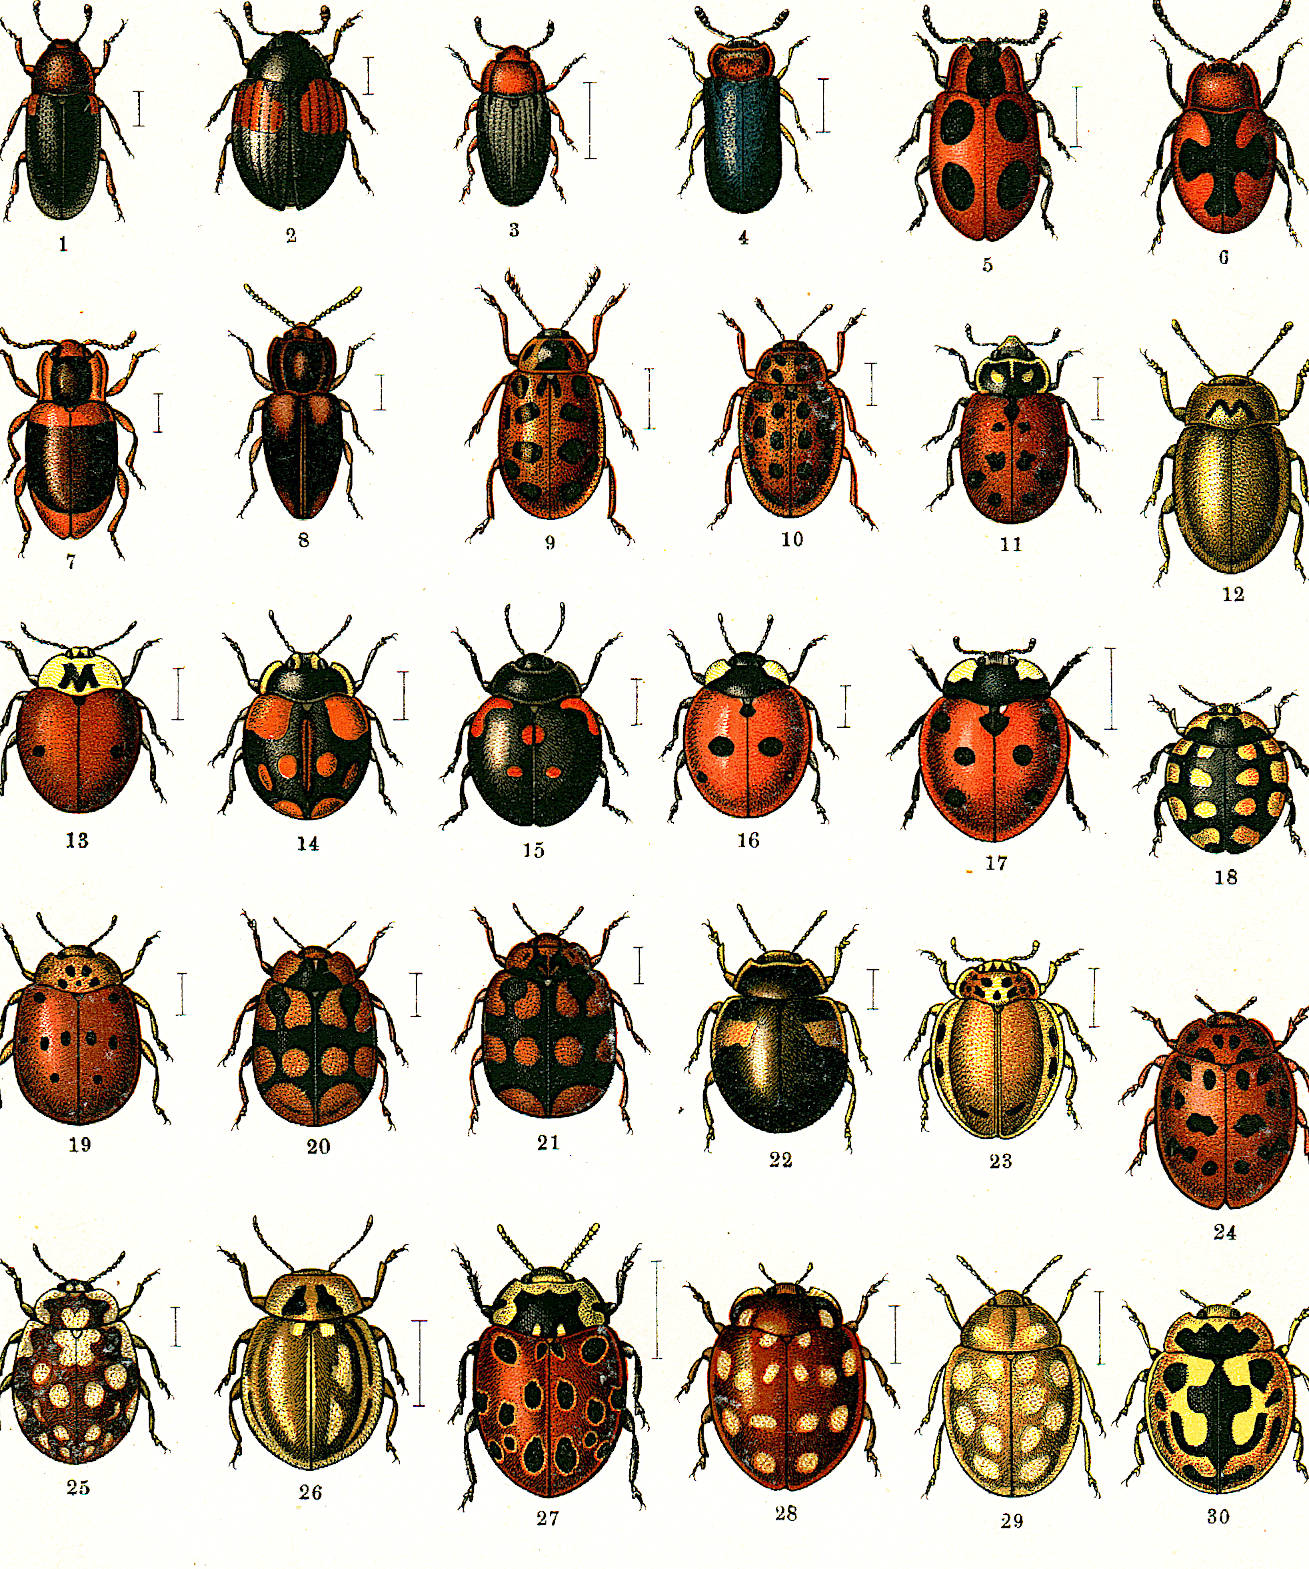
\includegraphics[width=\textwidth]{media/beetles_small.jpg}
		\end{columns}
	\end{frame}

	\begin{frame}{Cerebellum Model -- Microcircuits}
		\centering
		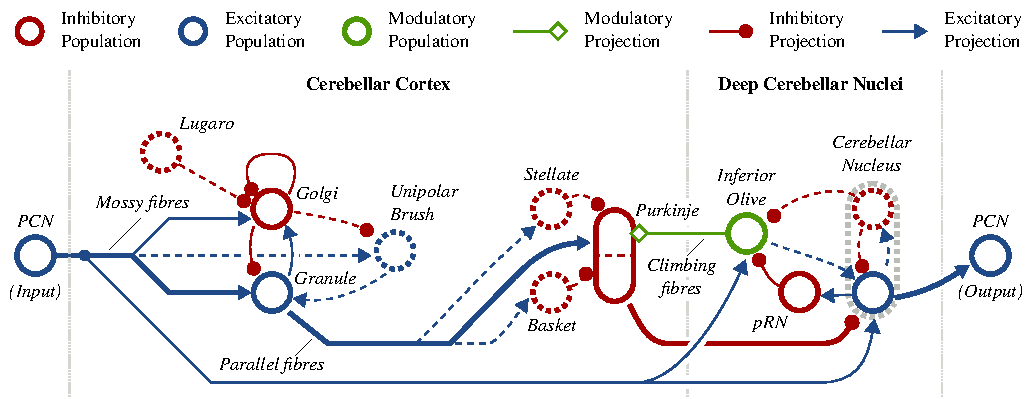
\includegraphics[width=\textwidth]{media/cerebellum_anatomy.pdf}
	\end{frame}

	\begin{frame}{Cerebellum Model -- Introduction}
		\begin{columns}[c]
			\column{0.5\textwidth}
			\begin{block}{\hl{Cerebellum}}
				\begin{itemize}
					\setlength{\itemsep}{0.5cm}
					\item Important for motor control
					\item Mostly Feed-Forward architecture
					\item May support cognitive tasks
					\item Model task: eyeblink conditioning
				\end{itemize}
			\end{block}
		\end{columns}
	\end{frame}

	\begin{frame}{Cerebellum Model -- Review: Classical Conditioning}
		\centering
		Before conditioning:\\[0.125cm]
		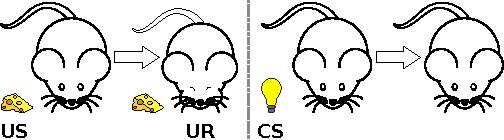
\includegraphics{media/classical_conditioning_a.pdf}\\[0.5cm]
		After conditioning:\\[0.125cm]
		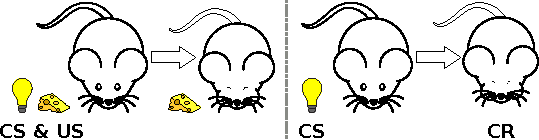
\includegraphics{media/classical_conditioning_b.pdf}\\[0.5cm]
		\ImageSources{Images adapted from \href{https://commons.wikimedia.org/wiki/File:Classical_conditioning_-_extinction.svg}{Wikimedia}.}
	\end{frame}
	
	\begin{frame}{Cerebellum Model -- Eyeblink Conditioning --- Experimental Setup}
		\centering\hspace*{-1cm}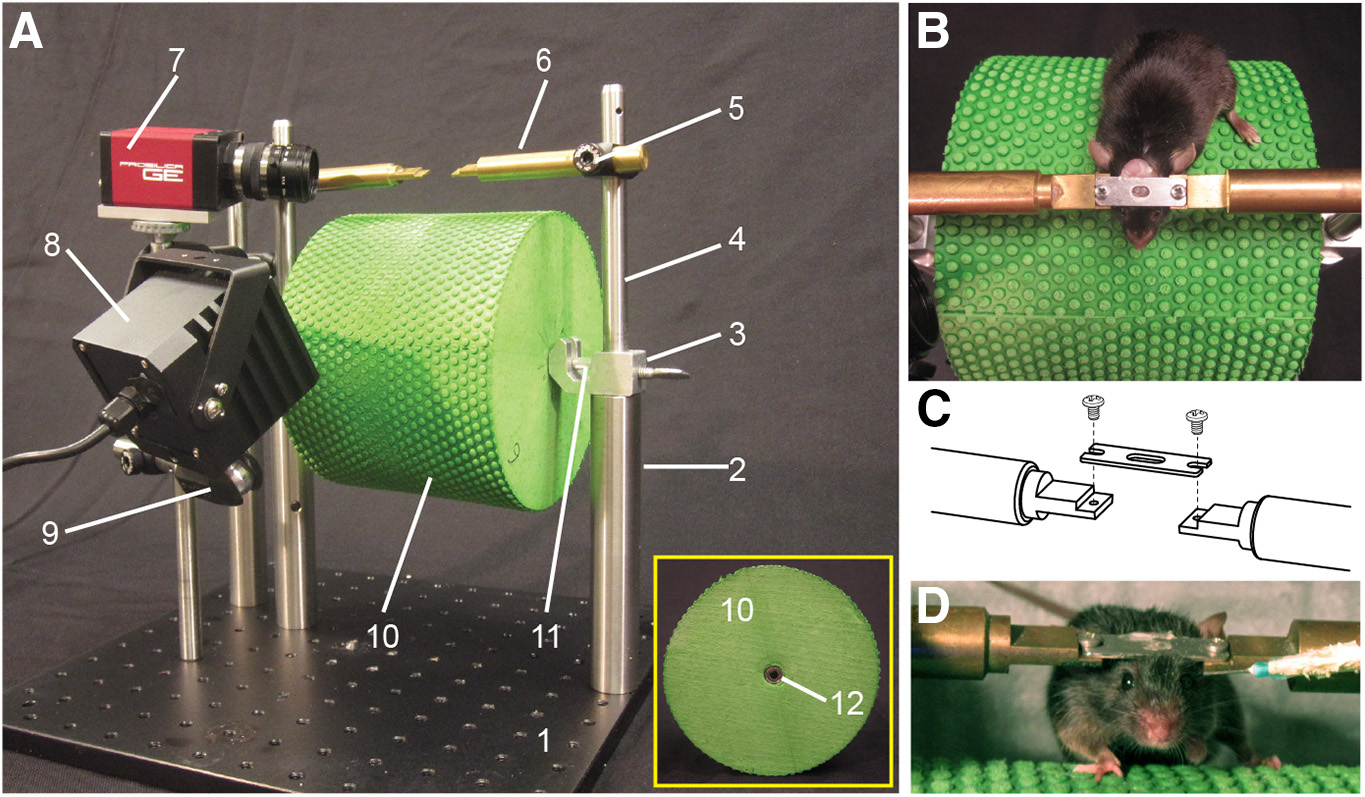
\includegraphics[height=0.725\textheight]{media/heiney_at_al_apparatus.png}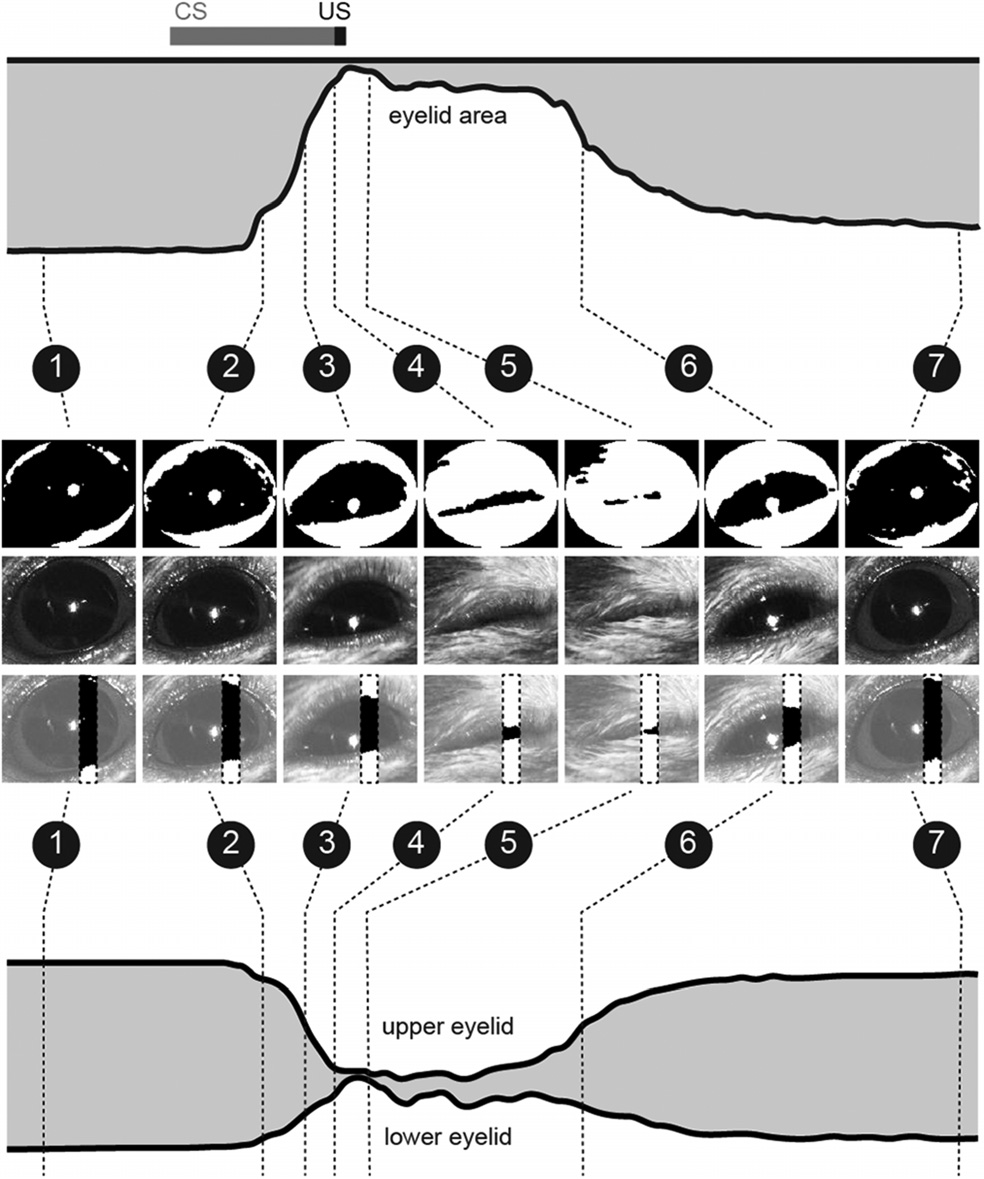
\includegraphics[height=0.725\textheight]{media/heiney_at_al_eyelid.png}
	\end{frame}
	
	\begin{frame}{Cerebellum Model -- Eyeblink Conditioning --- Data}
		\centering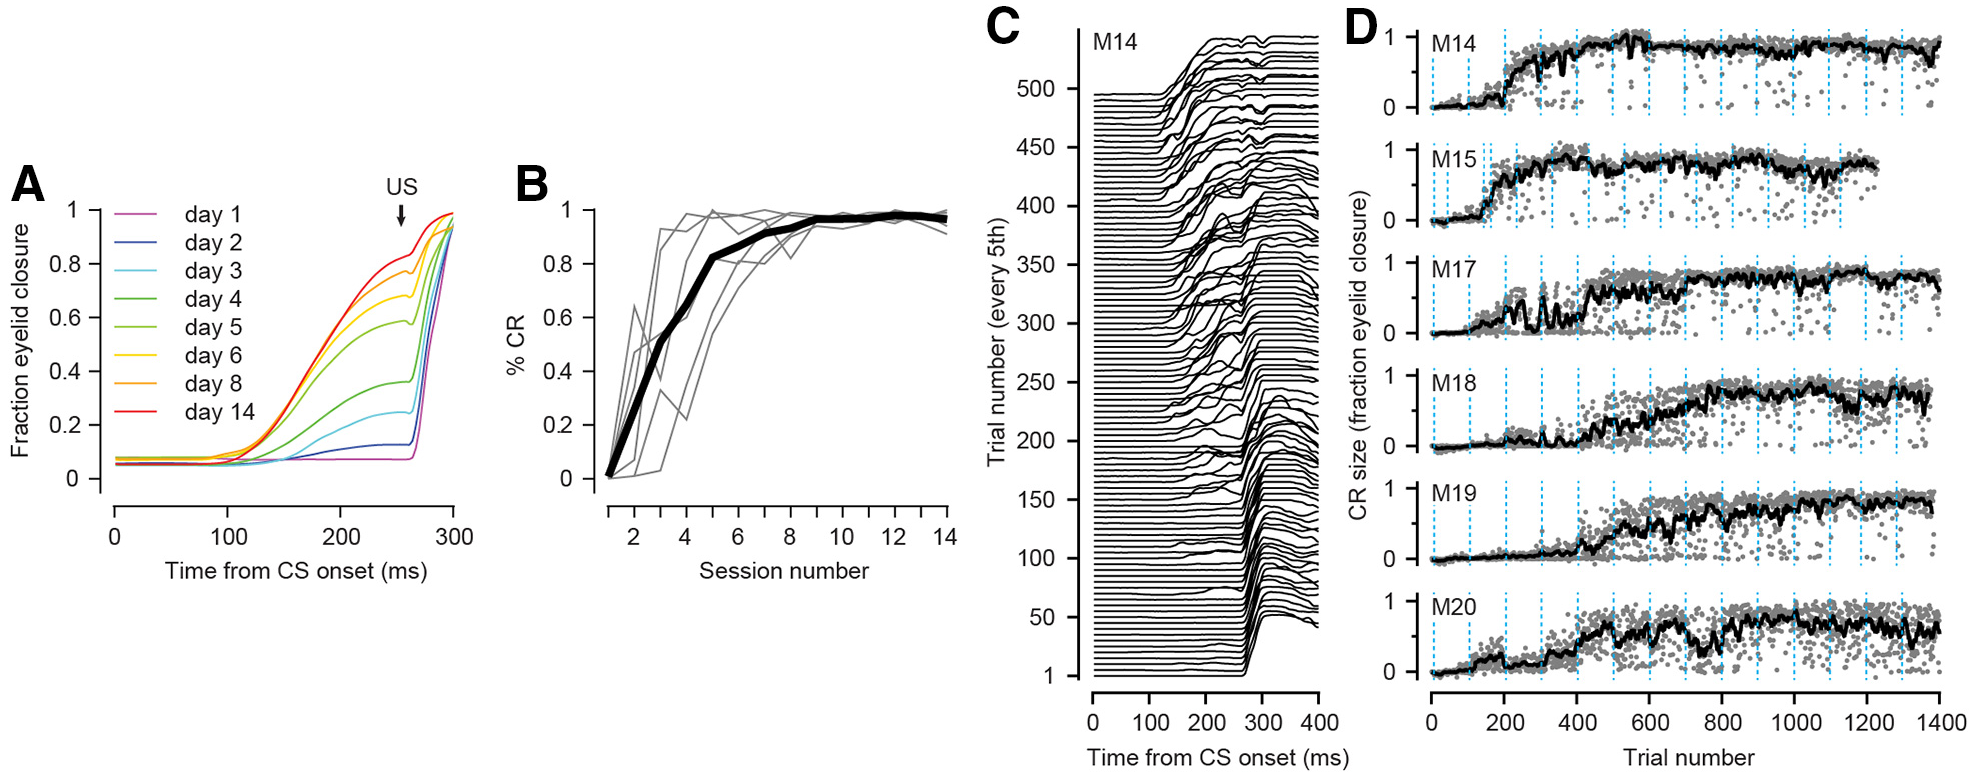
\includegraphics[width=\textwidth]{media/heiney_et_al_avg_cr_over_time_2.png}
	\end{frame}
	
	\begin{frame}{Cerebellum Model -- Open Questions: How are Delays Learned?}
		\begin{columns}[t]
			\column{0.5\textwidth}
			\centering
			\hl{Hypothesis 1}\\[0.25cm]
			\enquote{Dynamics Representation}/\\\enquote{Adaptive Filter Hypothesis}\\[0.775cm]
			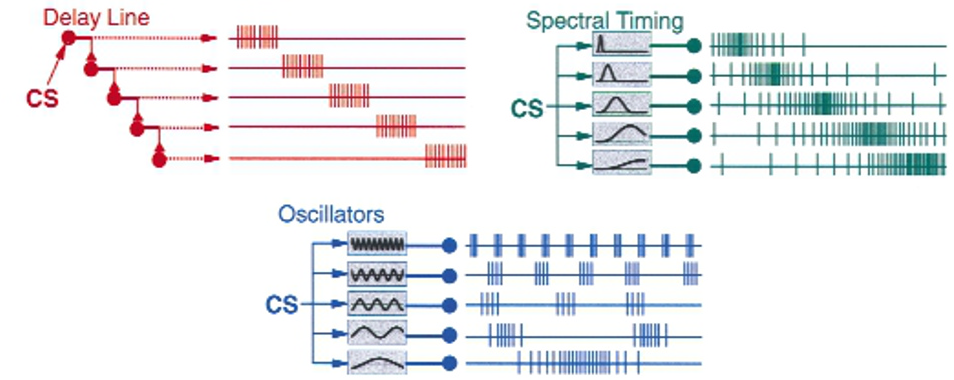
\includegraphics[width=\textwidth]{media/dynamics_rep.png}\\[0.775cm]
			Maybe dynamics are produced in the recurrent Granule-Golgi connection?
			\column{0.5\textwidth}
			\centering
			\hl{Hypothesis 2}\\[0.25cm]
			\enquote{Intrinsic Neural Properties}\\[0.25cm]
			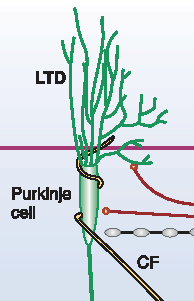
\includegraphics[width=0.4\textwidth]{media/purkinje.pdf}\\[0.25cm]
			Maybe the Purkinje cells are able to learn timings?
		\end{columns}
	\end{frame}
	
	\begin{frame}{Cerebellum Model -- The Delay Network}
		\centering
		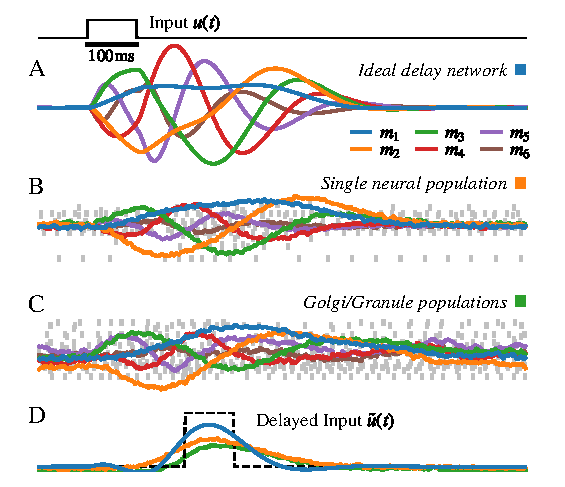
\includegraphics[height=0.8\textheight]{media/delay_network_response.pdf}
	\end{frame}
	
	\begin{frame}{Cerebellum Model -- Implementing The Delay Network}
		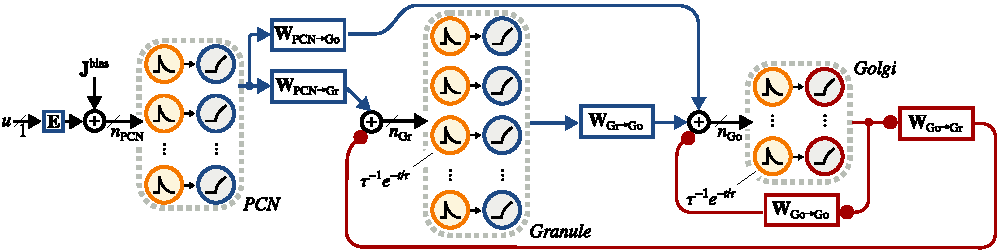
\includegraphics[width=\textwidth]{media/delay_network_dale.pdf}
	\end{frame}
	
	\begin{frame}{Cerebellum Model -- Experiment \& Results}
		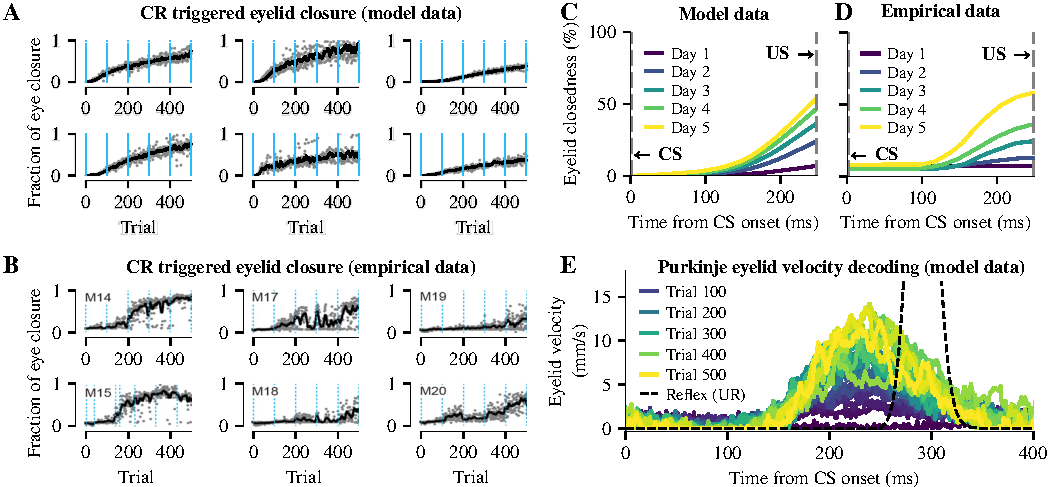
\includegraphics[width=\textwidth]{media/results_panel.pdf}
	\end{frame}

	\begin{frame}{Review -- Neuron Models}
		\centering%
		\vspace{0.125cm}%
		\includegraphics<1>[scale=0.95]{media/nonlinearities_01.pdf}%
		\includegraphics<2>[scale=0.95]{media/nonlinearities_02.pdf}%
		\includegraphics<3>[scale=0.95]{media/nonlinearities_03.pdf}%
		\includegraphics<4>[scale=0.95]{media/nonlinearities_04.pdf}%
		\includegraphics<5>[scale=0.95]{media/nonlinearities_05.pdf}%
		\includegraphics<6>[scale=0.95]{media/nonlinearities_06.pdf}%
		%\includegraphics<7>[scale=0.95]{media/nonlinearities_07.pdf}%
		%\includegraphics<7>[scale=0.95]{media/nonlinearities_08.pdf}%
		\includegraphics<7>[scale=0.95]{media/nonlinearities_09.pdf}%
	\end{frame}

	\begin{frame}{Conductance-Based Synapses -- Neuron Model}
		\centering
		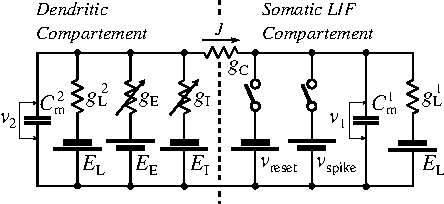
\includegraphics[scale=1.25]{media/neuron_model.pdf}
	\end{frame}

	\begin{frame}{Synaptic Nonlinearity Function}
		\centering
		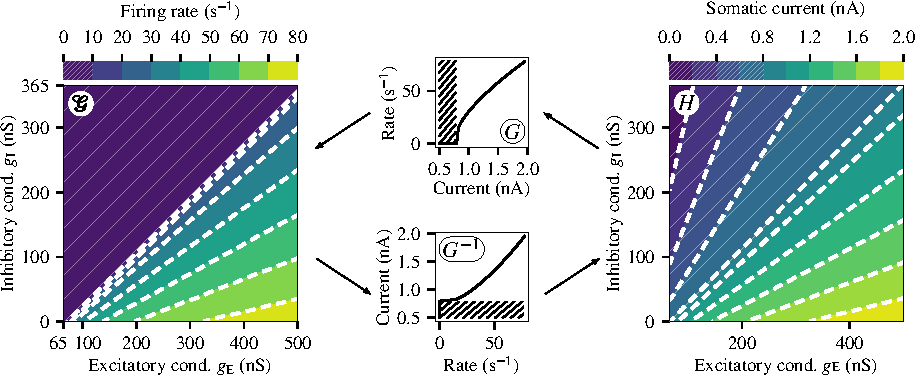
\includegraphics[width=\textwidth]{media/two_compartment_response_curve.pdf}
	\end{frame}

	\begin{frame}{Conductance-Based Synapses -- Dendritic Computation Experiment (I)}
		\textbf{Compute various two-dimensional functions}
		\begin{columns}
			\column{0.34\textwidth}
			\begin{itemize}
				\item Domain $(x, y) \in [0, 1]^2$
			\end{itemize}
			\column{0.36\textwidth}
			\begin{itemize}
				\item 100 neurons per population
			\end{itemize}
			\column{0.3\textwidth}
			\begin{itemize}
				\item Three topologies
			\end{itemize}
		\end{columns}
		\vspace{1cm}
		\begin{columns}
			\column{0.33\textwidth}
			\centering
			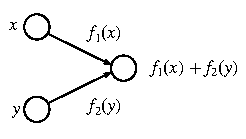
\includegraphics{media/network_a.pdf}\\
			\textbf{(a)} Additive network
			\column{0.33\textwidth}
			\centering
			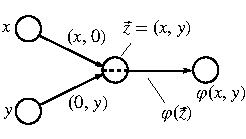
\includegraphics{media/network_c.pdf}\\
			\textbf{(b)} Intermediate layer
			\column{0.33\textwidth}
			\centering
			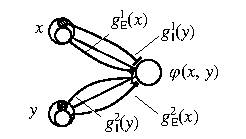
\includegraphics{media/network_d.pdf}\\
			\textbf{(c)} Synaptic computation
		\end{columns}
	\end{frame}


	\begin{frame}{Conductance-Based Synapses -- Dendritic Computation Experiment (II)}
		\centering
		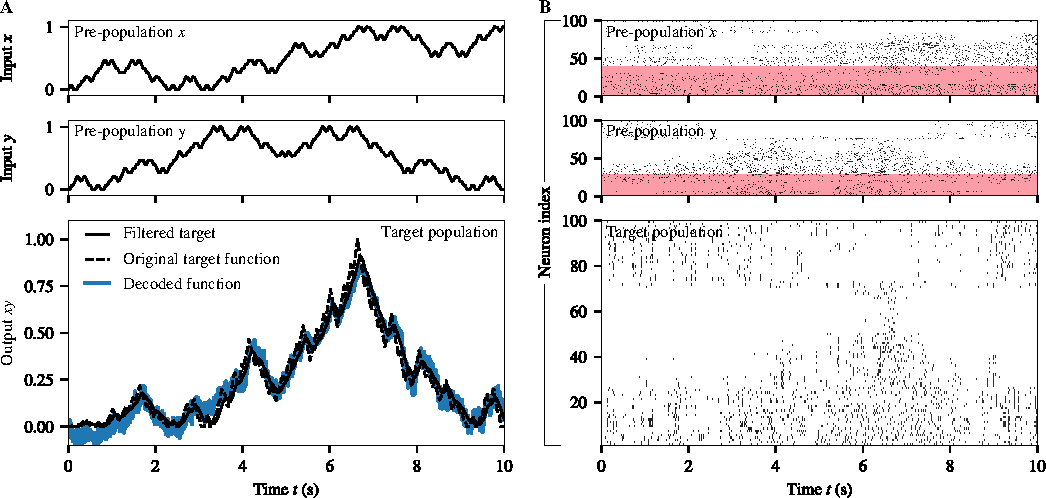
\includegraphics[width=\textwidth]{media/results_example.pdf}
	\end{frame}

	\begin{frame}{Conductance-Based Synapses -- Dendritic Computation Experiment (III)}
		\centering
		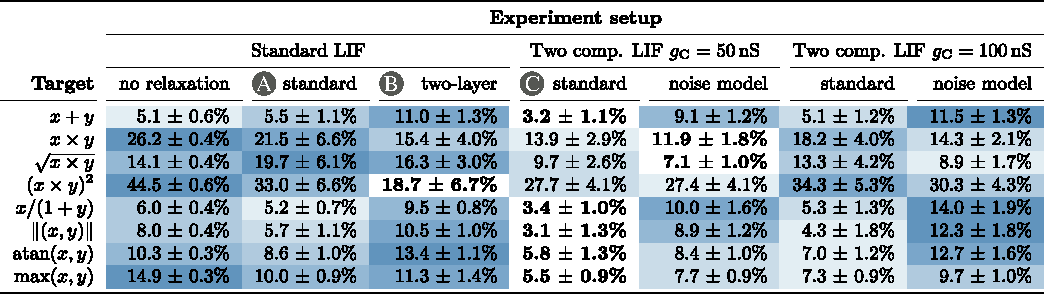
\includegraphics[width=\textwidth]{media/result_table.pdf}
	\end{frame}

	\backupbegin

	\begin{frame}[noframenumbering]{Image sources}
		\small
		\textbf{Title slide}\\Illustration of monographs Georgiy Jacobson "Beetles Russia and Western Europe"\\Around 1905\\ \href{https://commons.wikimedia.org/wiki/File:Jacobs24.jpg}{Wikimedia}.
	\end{frame}

	\backupend
	
\end{document}
